\chapter{Methods}
\maxdeadcycles=200

\section{Fathi Rabbani / 1164074}
\subsection{Teori}
\begin{enumerate}
\item Random Forest
\subitem
Random forest  adalah suatu algoritma yang digunakan pada klasifikasi data dalam jumlah yang besar. Klasifikasi random forest dilakukan melalui penggabungan pohon (tree) dengan melakukan training pada sampel data yang dimiliki. Penggunaan pohon (tree) yang semakin banyak akan mempengaruhi akurasi yang akan didapatkan menjadi lebih baik. Penentuan klasifikasi dengan random forest diambil berdasarkan hasil voting dari tree yang terbentuk. Pemenang dari tree yang terbentuk ditentukan dengan vote terbanyak. berikut adalah struktur dari Random Forest ada pada Gambar \ref{fig1}

\item Membaca Dataset, Makna setiap file dan Menjelaskan data CUB-200-2011
\begin{enumerate}
\item Membaca Data
\begin{itemize}
\item
dengan membuka data yang sudah didownload yaitu data CUB-200-2011 atau data tentang perbandingan data jenis burung,
\item
lalu data tersebut dibuka dengan menggunakan aplikasi Spyder, dan dijalankan setiap baris Code yang ada.
\item data yang ada pada folder CUB-200-2011 dibuka dengan menggunakan code dari Chapter 2 yang ada pada buku pembelajaran.
\end{itemize}

\item Makna setiap File
\begin{itemize}
\item data yang terdapat pada file CUB-200-2011 ada data folder ATTRIBUTE, IMAGES, PARTS yang memiliki kegunaannya sendiri yang dimana pada penggunaannya data yang dipakai adalah data image\_attribute\_label pada folder attribute, data image\_class\_labels dan data classes.
\item file image\_attribute\_label berguna sebagai data awal yang digunakan untuk membaca data attribute yang terdapat pada masing - masing gambar burung yang ada.
\item sedangkan file image\_class\_label yang ada pada folder CUB-200-2011 berguna sebagai data yang akan membuat kolom baru pada dataset yang fungsinya adalah untuk memasukan hasil dari semua data yang dimiliki oleh imgatt2.
\item dan file classes berguna sebagai dataset yang akan dipanggil oleh fungsi code untuk menampilkan nama dari data burung yang dimiliki.
\end{itemize}

\item Isi Field
\begin{itemize}
\item file image\_attribute\_label
berisi tentang data attribute yang ada pada data gambar file burung yang dimiliki difolder image pada CUB-200-2011
\item file image\_class\_label
berisi tentang data yang dimiliki oleh attribute dari image\_attribute\_label dimana data yang bernilai atau memiliki nilai disusun hingga menghasilkan data yang mudah dipahami.
\item file classes
berisi tentang data yang berguna untuk menampilkan data nama dari setiap data jenis burung yang dimiliki.
\end{itemize}
\end{enumerate}

\item Cross Validation
\subitem
Cross-validation adalah metode statistik yang dapat digunakan untuk mengevaluasi kinerja model atau algoritma dimana data dipisahkan menjadi dua subset yaitu data training dan data testing.

\item Score 44 Random Forest, 27 Decision Tree dan 29 SVM
\begin{enumerate}
\item
merupakan hasil dari pengolahan tentang data jenis burung yang dimiliki setelah melalui proses pembagian data training dan testing yang menghasilkan score 44 persen sebagai pembanding bahwa data yang diolah tersebut bernilai 44 persen tingkat kebenarannya atau keakuratannya.
\item
lalu pada penggunaan decision tree yang menghasilkan nilai 27 persen menjelaskan bahwa data yang diolah dengan menggunakan decision tree sebagai fungsi pembandingannya itu lebih kecil tingkat keakuratan hasilnya yang dimana kita mencari keakuratan data dari setiap jenis burung yang ada.
\item
sedangkan dengan menggunakan SVM menghasilkan nilai sebesar 29 persen yang dimana merupakan nilai nertal menjelaskan bahwa data yang diolah masih belum akurat tingkat kesamaannya dengan data jenis burung yang dimiliki.
\end{enumerate}
dari penjelasan tersebut disimpulkan bahwa penggunaan randowm forest dalam menentukan keakuratan data itu lebih besar scorenya dibandingkan menggunakan decision tree dan SVM.

\item Membaca Confusion Matriks
\begin{verbatim}
import numpy as np
np.set_printoptions(precision=2)
plt.figure(figsize=(60,60), dpi=300)
plot_confusion_matrix(cm, classes=birds, normalize=True)
plt.show()
\end{verbatim}
penggunaan code diatas adala cara untuk membaca dataset jenis burung dengan metode confusion matriks. dimana contoh hasil dari membaca data dengan menggunakan confusion matriks adalah sebagai berikut : Gambar \ref{fig2}

\item Voting pada Random Forest
voting pada random forest berguna untuk mengambil nilai yang akan digunakan sebagai bandingan dari masing - masing tree yang ada untuk menghasilkan nilai final sebagai data yang diinginkan, contohnya adalah seperti berikut ini : Gambar \ref{fig3}
\end{enumerate}

\subsection{Praktek}
\begin{enumerate}
\item membaca data Hero Dota dengan Pandas
\subitem
pada code ini akan dijelaskan maksud dan tujuan dari setiap baris code yang ada.
\begin{itemize}
\item pertama ada perintah import yang berguna untuk memanggil library pandas untuk digunakan aliaskan sebagai dota agar mudah dalam melakukan pemanggilan variable.
\item lalu ada variable hero yang menampung data untuk ditampilkan.
\item lalu ada variable dh yang berguna sebagai variable yang akan memanggil proses dari data dota dengan menggunakan tipe DataFrame dengan data variable hero.
\item lalu perintah print untuk menampilkan hasilnya ada pada gambar \ref{p1}.
\end{itemize}

\item membaca data Integer yang disusun dengan menggunakan Numpy
\subitem 
pada code ini kita akan menggunakan numpy sebagai library dengan beberapa function codenya seperti eye(), reshape() dan dot(), langsung saja dijelaskan bagian dari masing - masing baris codenya.
\begin{itemize}
\item pertama ada import numpy as cat dengan menggunakan library numpy maka kita harus terlebih dahulu melakukan import librarynya agar dapat menggunakan function yang terdapat disana, lalu kita menggunakan aliasnya menjadi cat
\item lalu terdapat beberapa variable yang dibuat yaitu a, b dan c dengan memiliki data tersendiri pertama ada variable a dengan function eye() yang berguna untuk menghasilkan matrix identitas, lalu disikan dengan nilai 5, hasilnya adalah sebagai berikut \ref{numpy21}.
\item lalu variable b dengan function arange dan reshape yang berguna untuk menyusun data menjadi 5 x 5 dengan jumlah data 25 hasilnya bisa dilihat pada gambar \ref{numpy22}
\item dan terakhir ada data variable c dengan function dot yang berguna untuk memberikan nilai titik pada masing - masing datanya seperti pada gambar \ref{numpy23}
\end{itemize}

\item membaca data variable dengan menggunakan Matplotlib 
\subitem 
pada code ini kita menggunakan matplotlib sebagai librarynya untuk dapat membaca data yang akan kita buat, pada kali ini kita akan menggunakan matplotlib dengan parameter class pyplot.
\begin{itemize}
\item pertama kita akan memanggil data metplotlibnya dengan menggunakan perintah import matplotlib.pyplot dengan alias me.
\item lalu pada code berikut terdapat 2 variable yaitu kecerdasan dan nilai untuk digunakan seabgai data acuan yang akan dibaca oleh function bar() dan akan ditampilkan dengan menggunakan function show() hasilnya adalah seperti pada gambar \ref{matplotlib}
\end{itemize}

\item Random Forest
\subitem
hasil yang didapatkan dari menggunakan pemrosesan data Random Forest terdapat pada gambar \ref{p1}, hasil dari keluarannya terdapat nilai 0.4553854276663147 yang jika kita masukan dalam proses ini menjadi 45 \% dengan nilai yang didapat tersebut meyakinkan bahwa data yang diolah telah mencapai titik dimana data tersebut dapat dianalisa dengan tepat.

\item Confusion Matrix
\subitem
hasil yang didapat dari proses menggunakan \ref{p2} confusion matrix adalah tampilnya gambar \ref{matrix} dengan hasil berupa gambar tersebut dapat dipastikan bahwa nilai yang didapatkan memiliki bebrapa titik yang dapat disusun seperti pada gambar berikut \ref{matrix2}.

\item Decision tree dan SVM
\begin{itemize}
\item Decision Tree
\subitem
hasil dari proses terdapat pada gambar \ref{p3} terdapat nilai 0.2713833157338965 yang diproses menjadi 27 \% pada kasus ini, yang menjelaskan bahwa nilai tersebut merupakan nilai dari hasil analisa function decision tree terhadap data yang sudah disediiakan.

\item SVM
\subitem
hasil dari proses terdapat pada gambar \ref{p4} terdapat nilai 0.28801478352692717 yang diproses menjadi 28 \% pada kasus ini, yang menjelaskan bahwa nilai tersebut merupakan nilai dari hasil analisa menggunakan function SVM terhadap data yang sudah disediiakan dan menghasilkan data tersebut.
\end{itemize}

\item Cross Validation
\subitem
pada hasil dari proses cross validation ini terdapat 3 hasil dengan menggunakan function Random Forest, Decision Tree dan SVM, yang menghasilkan beberapa data yang terdapat pada gambar \ref{p5} sebagai data nilai Random Forest, \ref{p6} sebagai hasil data Decision tree dan \ref{p7} merupakan hasil dari SVM. dimana data pada Random Forest bernilai 0.44 , Decision Tree 0.26 dan SVM 0.26 yang berarti dari 3 function yang digunakan untuk melakukan analisa data penggunaan Random Forest lah yang menghasilkan nilai data paling signifikan sehingga data yang diolah dapat diketahui bahwasannya data tersebut sudah 44 \% termasuk data valid atau benar.

\item Pengamatan
pengamatan hasil data tersebut dibagi menjadi 2 yaitu dengan metode cross validation dan matplotlib, hasilnya adalah sebagai berikut ini :
\begin{itemize}
\item Cross Validation
\subitem
data yang dihasilkan merupakan data pengamatan apakah nilai yang dikeluarkan merupakan nilai yang valid sehingga data yang dianalisa dapat diketahui kebenarannya dengan menggunakan nilai range10 - 200 dengan lompatan 20 data dan dimulai dari 10 serta 5 perulangan data hasilnya sebanyak 50 kali, hasilnya terdapat pada gambar \ref{p8}
\item Matplotlib
\subitem
data yang dihasilkan merupakan data pengamatan apakah nilai yang dikeluarkan merupakan nilai yang valid sehingga data yang dianalisa dapat diketahui kebenarannya dengan menggunakan class Axes3D yang akan menghasilkan data berupa gambar\ref{p8} dimana data yang terbaca adalah menggunakan nilai variable X Y Z dengan membandingkan nilai dari masing - masing data varible tersebut, hasilnya terdapat pada gambar \ref{p8}
\end{itemize}
\end{enumerate}

\subsection{Error}
\begin{enumerate}
\item Error pada gambar \ref{error}
\item Jenis Error adalah tidak terbacanya data karena kurangnya nilai yang dimasukan
\item Solusinya adalah dengan menambahkan nilai sesuai dengan jumlah masing - masing kolom hasilnya ada pada gambar \ref{fix}
\end{enumerate}


\begin{figure}
	\centerline{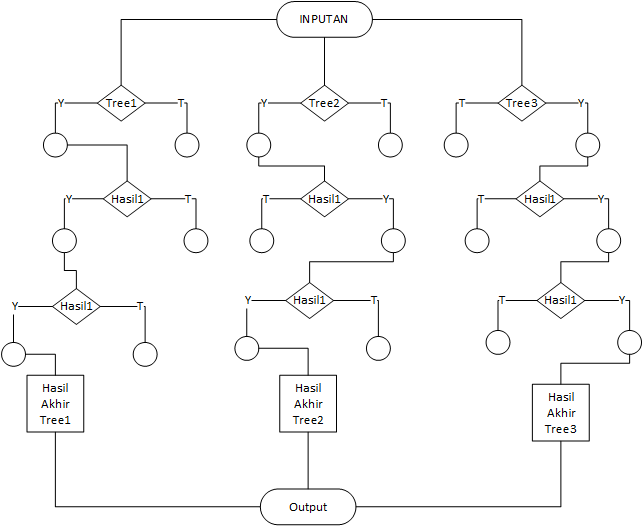
\includegraphics[width=1\textwidth]{figures/fathi/chapter3/hari1/1.png}}
	\caption{Random Forest}
	\label{fig1}
\end{figure}

\begin{figure}
	\centerline{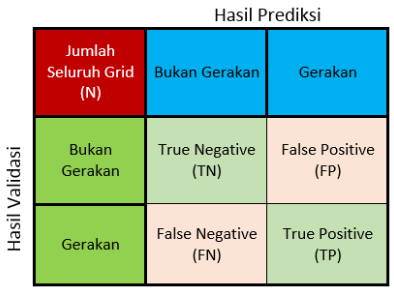
\includegraphics[width=1\textwidth]{figures/fathi/chapter3/hari1/2.PNG}}
	\caption{Hasil dari membaca data dengan Confusion Matriks}
	\label{fig2}
\end{figure}

\begin{figure}
	\centerline{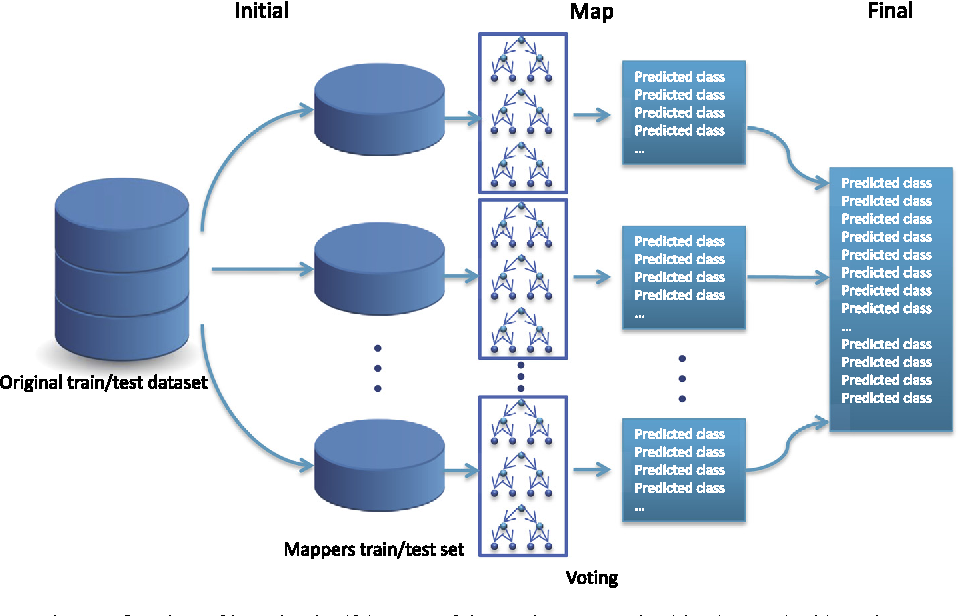
\includegraphics[width=1\textwidth]{figures/fathi/chapter3/hari1/3.png}}
	\caption{Voting Random Forest}
	\label{fig3}
\end{figure}

\begin{figure}
	\centerline{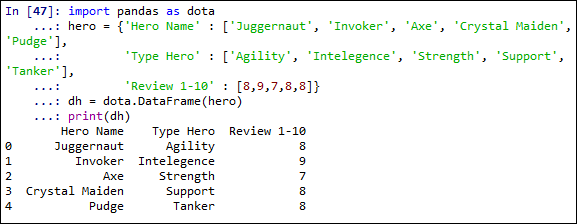
\includegraphics[width=1\textwidth]{figures/fathi/chapter3/hari2/1.png}}
	\caption{Pandas Implementasi}
	\label{pandas}
\end{figure}

\begin{figure}
	\centerline{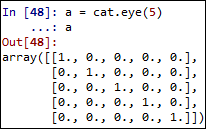
\includegraphics[width=1\textwidth]{figures/fathi/chapter3/hari2/21.png}}
	\caption{Numpy Implementasi}
	\label{numpy1}
\end{figure}

\begin{figure}
	\centerline{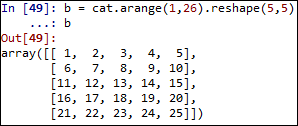
\includegraphics[width=1\textwidth]{figures/fathi/chapter3/hari2/22.png}}
	\caption{Numpy Implementasi}
	\label{numpy2}
\end{figure}

\begin{figure}
	\centerline{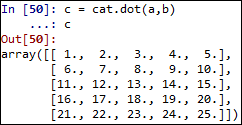
\includegraphics[width=1\textwidth]{figures/fathi/chapter3/hari2/23.png}}
	\caption{Numpy Implementasi}
	\label{numpy3}
\end{figure}

\begin{figure}
	\centerline{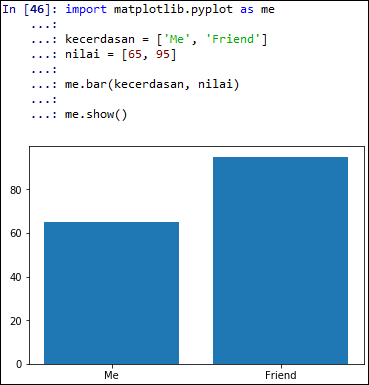
\includegraphics[width=1\textwidth]{figures/fathi/chapter3/hari2/3.png}}
	\caption{Matplotlib Implementasi}
	\label{matplotlib}
\end{figure}

\begin{figure}
	\centerline{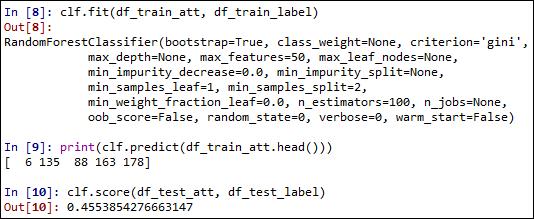
\includegraphics[width=1\textwidth]{figures/fathi/chapter3/hari2/4.png}}
	\caption{Random Forest Classifier}
	\label{p1}
\end{figure}

\begin{figure}
	\centerline{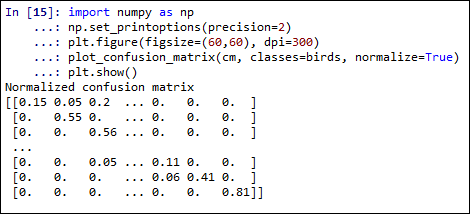
\includegraphics[width=1\textwidth]{figures/fathi/chapter3/hari2/5.png}}
	\caption{Confusion Matrix}
	\label{p2}
\end{figure}

\begin{figure}
	\centerline{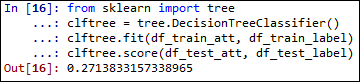
\includegraphics[width=1\textwidth]{figures/fathi/chapter3/hari2/6.png}}
	\caption{Decision Tree}
	\label{p3}
\end{figure}

\begin{figure}
	\centerline{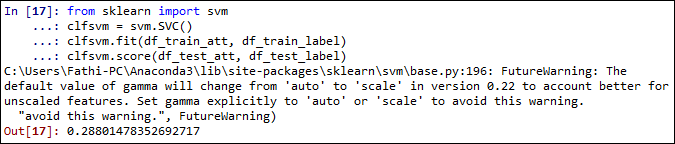
\includegraphics[width=1\textwidth]{figures/fathi/chapter3/hari2/7.png}}
	\caption{Support Vector Machine}
	\label{p4}
\end{figure}

\begin{figure}
	\centerline{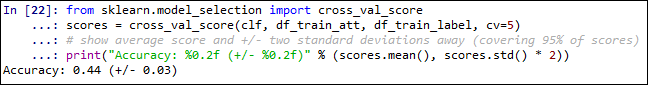
\includegraphics[width=1\textwidth]{figures/fathi/chapter3/hari2/8.png}}
	\caption{Cross Validation data Random Forest}
	\label{p5}
\end{figure}

\begin{figure}
	\centerline{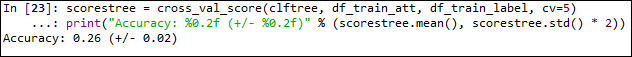
\includegraphics[width=1\textwidth]{figures/fathi/chapter3/hari2/9.png}}
	\caption{Cross Validation data Decision Tree}
	\label{p6}
\end{figure}

\begin{figure}
	\centerline{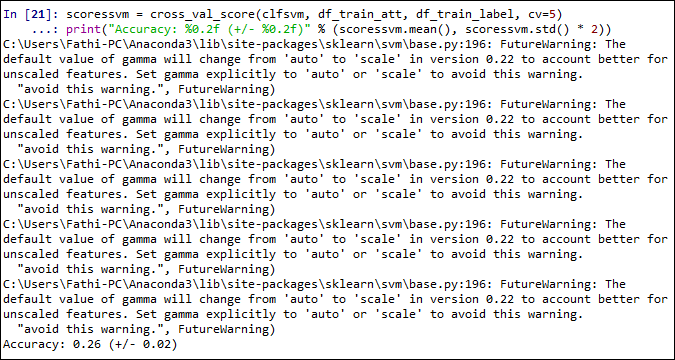
\includegraphics[width=1\textwidth]{figures/fathi/chapter3/hari2/10.png}}
	\caption{Cross Validation data SVM}
	\label{p7}
\end{figure}

\begin{figure}
	\centerline{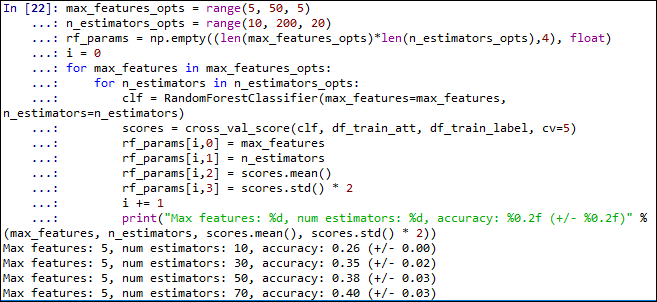
\includegraphics[width=1\textwidth]{figures/fathi/chapter3/hari2/11.png}}
	\caption{Pengamatan Akurasi data dengan Cross Validation}
	\label{p8}
\end{figure}

\begin{figure}
	\centerline{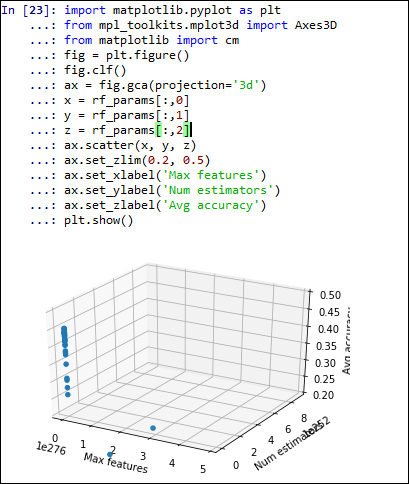
\includegraphics[width=1\textwidth]{figures/fathi/chapter3/hari2/12.png}}
	\caption{Pengamatan Akurasi data dengan Matplotlib}
	\label{p9}
\end{figure}

\begin{figure}
	\centerline{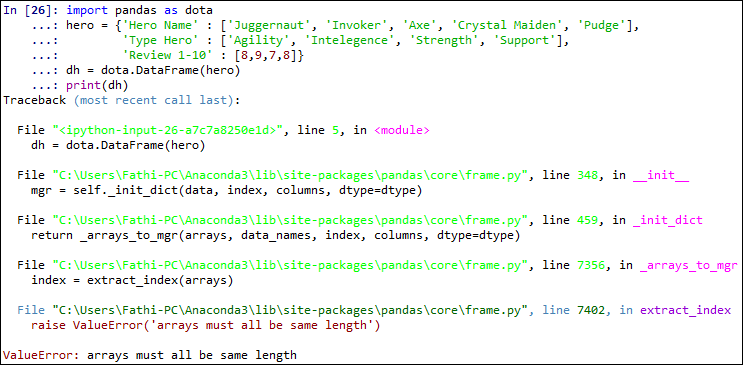
\includegraphics[width=1\textwidth]{figures/fathi/chapter3/hari2/error.png}}
	\caption{Cross Validation data Random Forest}
	\label{error}
\end{figure}

\begin{figure}
	\centerline{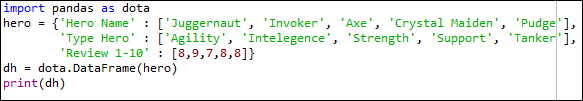
\includegraphics[width=1\textwidth]{figures/fathi/chapter3/hari2/fix.png}}
	\caption{Cross Validation data Random Forest}
	\label{fix}
\end{figure}

\begin{figure}
	\centerline{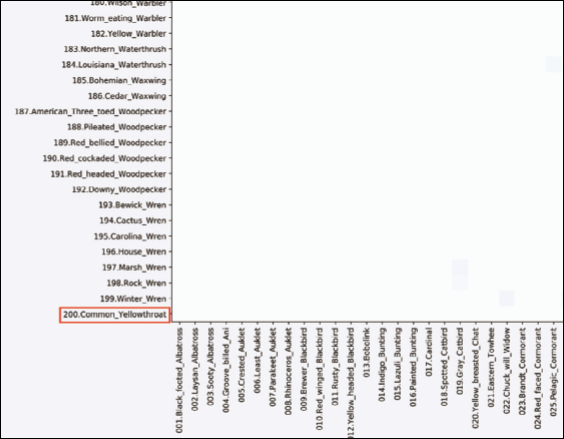
\includegraphics[width=1\textwidth]{figures/fathi/chapter3/hari2/matrix.png}}
	\caption{Hasil Confusion Matrix}
	\label{matrix}
\end{figure}

\begin{figure}
	\centerline{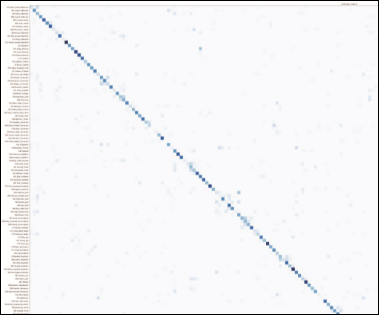
\includegraphics[width=1\textwidth]{figures/fathi/chapter3/hari2/matrix2.png}}
	\caption{Hasil Confusion Matrix}
	\label{matrix2}
\end{figure}


\section{Cokro Edi Prawiro / 1164069}

\subsection{Teori}
\begin{enumerate}
\item Jelaskan apa itu random forest, sertakan gambar ilustrasi buatan sendiri.\par
Random Forest atau hutan acak yaitu kumpulan dari pohon-pohon keputusan yang digunakan untuk membaca objek tertentu yang telah di sepakati untuk di baca dalam AI. pohon-pohon keputusan tersebut akan memunculkan hasil-hasil yang akan disimpulkan oleh random forest. pembagian jumlah data yang dimasukan kedalam decision tree pada random forest akan di bagi sama rata sesuai codingan atau ketentuan tertentu yang di sepakati. misalkan data yang akan digunakan sebanyak 314 jika dalam satu decision tree di putuskan untuk memiliki 50 data maka pada satu random forest akan terdapat enam atau tujuh decision tree. untuk lebih jelasnya dapat dilihat pemisalan pada gambar \ref{c36} random forest berikut.


\item Jelaskan cara membaca dataset khusus dan artikan makna setiap file dan isi field masing masing file.
langkah pertama download terlebih dahulu dataset nya kemudian buka menggunakan spyder bawaan anaconda untuk mengetahui isi dari dataset tersebut. biasanya data tersebut berisi databerekstensi .txt yang di dalammya terdapat class dari field atau data data yang ada data tersebut. contoh pada data burung ada field index dan angka, index biasanya berisi angka, angka angka tersebut memiliki makna yaitu pengganti nama atau jenis dari burung tersebut sedangkan pada field yang berisi nilai 0 dan 1 berarti menyatakan atau maknanya yaitu memberikan nilai ya dan tidak nilai tersebut di ubah menjadi angka nol dan satu karna data pada field tersebut harus berisi nilai boolean atau pilihan ya dan tidak di karenakan komputer susah membaca nilai dan tidak maka di ubahlah menjadi 0 dan 1 dengan 0 bernilai tidak dan 1 bernilai ya.

\item Jelaskan apa itu Cross Validation.
Cross Validation merupakan cara untuk mengevaluasi hasil dari sebuah metode yang telah digunakan dengan cara membagi dua bagian dari dataset menjadi data training dan data testing kemudian data tersebut diolah hingga muncul tingkat akurasi dari metode yang digunakan contoh pada metode random forest dataset nya di bagi menjadi dua menjadi data training dan data testing kemudian data tersebut di olah oleh mesin untuk melihat tingkat akurasinya maka akan muncul misalkan akurasi kebenaran sebesar 44 \% begitu pula dengan menggunakan metode-metode yang lain seperti decision tree dan SVM.


\item Jelaskan apa arti score 44 \% pada random forest, 27 \% pada decision tree dan 29 \% dari SVM.
maksud dari score 44 \% tersebut yaitu nilai ketepatan atau kebenaran atau bisa disebut hasil dari random forest misalkan dengan metode random forest mesin membaca objek burung, mesin tersebut bisa menyatakan jenis burung tersebut dengan akurasi kebenaran 44 \%. sedangkan pada metode decision tree yaitu 27 \% yang berarti menunjukan bahwa tingkat akurasi ketepatan mesin jika mengerjakan sesuatu atau menyatakan keputusan dengan metode decision tree maka nilai kebenarannya bernilai 27 \%. sedangkan dengan menggunakan metode SVM menunjukan hasil 29 \% yang berarti nilai ketepatan atau kebenaran dalam memecahkan masalah menggunakan metode SVM ini sebesar 29 \% . maka dari itu dapat di simpulkan bahwa dengan menggunakan metode random forest mesin dapat memecahkan masalah lebih akurat dibandingkan dengan menggunakan decision tree dan SVM.


\item Jelaskan bagaimana cara membaca confusion matriks dan contohnya memakai gambar atau ilustrasi sendiri.
cara membaca confusioo matrix dengan cara memasukan para meter nilai yang ada pada datasets contoh pada dataset terdapat class yang disandingkan dengan nama burung untuk di normalisasi maka akan menunjukan nilai matrix yang mendekati nilai benar dalam bentuk angka misalkan 0,5 0,2 dan seterusnya mendekati nilai satu. di karenakan susahnya membaca nilai angka maka sering di ubah menjadi bentuk grafik. dapat di lihat pada gambar \ref{c38}


\item Jelaskan apa itu voting pada random forest disertai dengan ilustrasi gambar sendiri.\par
Voting merupakan data hasil dari decision tree yang terdapat pada random forest. Dimana hasil data tersebut di gunakan sebagai acuan untuk hasil dari random forest. sebagai contoh misalkan pada satu random forest terdapat enam decision tree untuk menentukan jenis pekerjaan orang, pada decision tree ke satu menyimpulkan bahwa pekerjaanya yaitu dosen , pada decision tree ke dua yaitu dosen kemudian pada decision tiga dosen , pada decision tree ke empat yaitu pekerja kantoran, pada decision tree ke lima yaitu pekerja kantoran dan pada decision tree ke enam yaitu dosen. maka pada random forest dapat menyimpulkan hasilnya yaitu dosen. untuk lebih jelasnya dapat dilihat pada gambar \ref{c37} . 

\end{enumerate}


\subsection{Praktikum}
\begin{enumerate}
\item pandas \par
arti tiap baris codingan yang terdapat pada gambar \ref{c39} yaitu. pada baris ke satu yaitu perintah mengimport library padas pada python atau anaconda kemudian di inisialisasikan menjadi kue. selanjutnya pada baris ke 3 terdapat nama variabel yaitu nama\_kue\_tradisional = yang di dalammyanya terdapat tiga nama field yakni Name Kue, harga satuan dan terbilang kemudian pada baris ke tujuh terdapat variabel baru bernama Data\_kue = kemudian didalammnya mendeskripsikan kue berdasarkan tipe DataFrame yang berisi variabel nama\_kue\_tradisional selanjutnya data tersebut di cetak pada console dengan perintah print (Data\_kue). untuk lebih jelasnya dapat dilihat pada gambar \ref{c39}. dan untuk hasilnya dapat dilihat pada gambar \ref{c40}

\item numpy\par
Arti tiap baris codingan pada aplikasi sederhana numpy adalah sebagai berikut : pada baris ke satu yaitu mengimport numpy yang di inisialisasi menjadi np kemudian pada baris ke tiga dibut variabel ali yang berisi numpy bertipekan arrange 6 yang berarti berisi nilai array dari 0 sampai 5 kemudian pada baris ke empat di cetak hasilnya dengan memasukan perintah print (ali) selanjutnya yaitu membuat nilai array tiga dimensi pada baris ke tujuh dengan cara membuat variabel botak yang berisi rank nilainya kemudian dimensinya yaitu 4 3 3 kemudian variabel tersebut di print. selanjutnya pada baris ke 12 dibuat variabel nilai\_array\_1 dengan isian nilai array 1 2 3 4 kemudian pada baris ke 13 di buat variabe nilai\_array\_2 dengan nilai array 20 30 40 dan 50 selanjutnya pada baris ke 14 dibut nilai variabel Nilai\_array\_3 dengan rank 4 yang berarti berisi nilai dari 0 sampai 3 setelah itu di buat variabel hasil dimana isinya yaitu penjumlahan nilai\_array\_1+Nilai\_array\_3+Nilai\_array\_3 setelah itu nilai\_array\_1 , Nilai\_array\_3, dan Hasil di prin untuk melihat nilai dari array tersebut. untuk lebih jelasnya codingan aplikasi sederhana numpy dapat dilihat pada gambar \ref{c41} berikut:

\item matplotlib\par
Arti tiap baris aplikasi sederhana matplotlib pada baris ke satu yaitu memasukan library matplotlib.pyplot yang di definisikan menjadi plt kemudian membuat variabel kelas\_ti3 pada baris ke tiga yang berisi label setelah itu di buat variabel jumlah\_mhs3 pada baris ke empat yang berisi nilai dari setiap label tersebut. begitu juga pada baris ke emam dan ke tujuh kemudian pada baris ke sembilan matplotlib mendefinisikan gambar dengan ukurannya dan pada baris ke 10 di dekralasikan subplot setelah itu pada baris ke 11 matplotlib mendefinisikan jenis grafik yang digunakan dan dimasukan variabel kelas dan jumlah\_mhs. begitujuga oada baris ke 13 14 dan 15 setelah itu di buat title  pada baris ke 17 dan matplotlib di show untuk mendapatkan hasil dari grafiknya. untuk lebih jelasnya dapat di lihat pada gambar\ref{c42} dan untuk hasilnya dapat dilihat pada gambar \ref{c43}.

\item Random Forest\par
Arti tiap baris hasil codingan random forest pada baris pertama random forest di import dari sklearn dengan ketentuan yaitu maksimal isi dari decision tree berisi 50 data dengan keadaan random dan dengan estimators 100 data ini berada dalam variabel clf kemudian setelah itu variabel clf di running berdasarkan data training dan data label yang telah di definisikan jumlahnya. kemudian variabel clf di running berdasarkan data training paling atas untuk memunculkan hasil data training lima paling atas. setelah itu data tersebut di di running scorenya untuk melihat tingkat akurasi yang dia kerjakan maka tingkat akurasi yang dihasilkan berada pada kisaran 0,437 atau kisaran 43 \%  untuk lebuh jelasnya dapat di lihat pada gambar \ref{c44} berikut.
 
\item Confusion Matrix\par
arti codingan pada hasil tiap codingan confusion matrix pada baris pertama codingan tersebut mendeskripsikan atau mengimport confusion matrix dari sklearn kemudian dibuat variabel pred labels dengan di isikan clf prdic df\_test\_att setelah itu membuat variabel cm yang isinya terdapat data yang di buat confusion matrix berdasarkan data test setelah variabel cm akan di running yang mana akan menghasilkan gambar berupa matrix matrix tersebut berisi nilai nilai kebenaran yang mendekati nilai benar atau mutlak nilai benar untuk hasilnya dapat di lihat pada gambar \ref{c45} data tersebut berisi data tipe int 64.

\item SVM dan Decision Tree\par
Arti dari setiap baris hasil codingan decision tree dan SVM pada tree masukan terlebih dahulu library tree setelah itu buat variabel clftree yang berisi decision tree setelah itu masukan nilai data training dan label yang telah di deklarasikan tadi setelah itu running variabel tersebut untuk mendapatkan score 0,266 kisaran 26 sampai 27 \% akurasinya kemudian pada svm juga hampirsama masukan terlebih dahulu librarynya setelah itu buat variabel clfsvm yang berarti berisi nilai data training dan data label dan pendeklarasian svm itu sendiri setelah itu di running untuk mendapatkan nilai akurasinya atau score sebesar 0,283 atau dalam kisaran 23 \%. untuk lebih jelasnya dapat di lihat pada gambar\ref{c46} sebagai berikut:

\item Cross Validation\par
arti dari setiap baris hasil cross falidation pada gambar\ref{c47} tersebut diperlihatkan codingan error dikarenakan data training terlalu besar maka untuk mengatasi halini dapat dlilihat pada sub bab penanganan error / cokro

\item program pengamatan
arti dari hasil program pengamatan. perogram pengamatan ini menggunakan library matplotlib supaya hasil dari presentase hasil random forest, svm dan decision tree dapat di bandingkan dengan membuat variabel X Y Z kemudian memberikan label untuk setiap dimensinya untuk lebih jelas dapat dilihat gambar \ref{c48} yang menunjukan hasil perbandingan presentase dari tiga metode tersebut. 
\end{enumerate}

\subsection{Penanganan Error / cokro}
Screenshot error
\begin{enumerate}
\item  Untuk gambar screenshot error yang pertama dapat dilihat pada gamabar \ref{c49}
\item  Untuk gambar screenshot error yang kedua dapat dilihat pada gamaba r\ref{c50}
\item  Untuk gambar screenshot error yang ketiga dapat dilihat pada gamabar \ref{c51}
\item  Untuk gambar screenshot error yang keempat dapat dilihat pada gamabar \ref{c52}
\end{enumerate}

Code Errornya 
\begin{enumerate}
\item kode error pada screenshot ke satu yaitu dikarenakan clfsvm.fit(df\_train\_att, df\_train\_label) dikarenakan data trainingnya terlalu besar sehingga komputernya error.
\item untuk kode error pada screen shoot ke 2 sampai ke 4 dikarenakan pada kode berikut  scores = cross\_val\_score(clf, df\_train\_att, df\_train\_label, cv=5) scorestree = cross\_val\_score(clftree, df\_train\_att, df\_train\_label, cv=5) dan  
scoressvm = cross\_val\_score(clfsvm, df\_train\_att, df\_train\_label, cv=5) hal ini di karenakan data trainingterlalu besar sehingga berdampak pada komputer sehingga library dari python tidak mampu mengolah data dan hasilnya menjadi error. 
\end{enumerate}

Solusi Untuk mengatasi Error
\begin{enumerate}
\item solusinya untuk yang ke satu yaitu dengan cara merestart spyder atau mematikannya kemudian nyalakan kembali setelah itu jalankan code yang error tersebut di CMD cika dalam python CMD jalam maka bisa di running. setelah itu buka kembali spyder dan jalankan codingan dari awal hingga pada bagian SVM tunggu sebenar sampai muncul nilai akurasinya.
\item solusi untuk mengatasi error tersebut yaitu dengan cara merubah bobot data pada data training seperti pada gambar \ref{c53}
setelah itu running code yang errornya maka akan muncul hasilnya dengan sekala yang lebih kecil dari persenan yang seharusnya. maka hasilnya seperti pada gambar \ref{c54} berikut.
\end{enumerate}


\begin{figure}
      \centerline{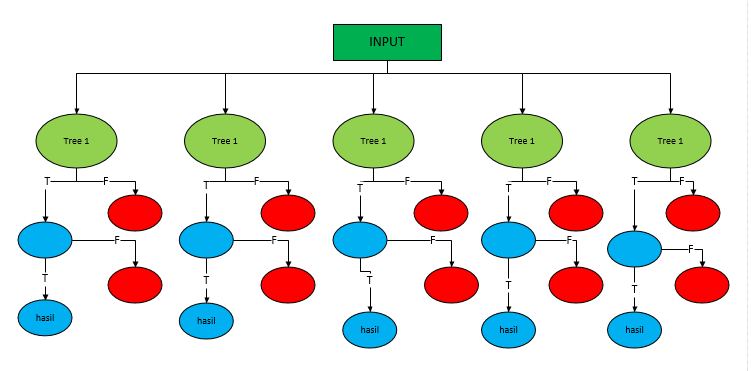
\includegraphics[width=1\textwidth]
      {figures/cokro/c36}}
      \caption{Random Forest}
      \label{c36}
      \end{figure}

\begin{figure}
      \centerline{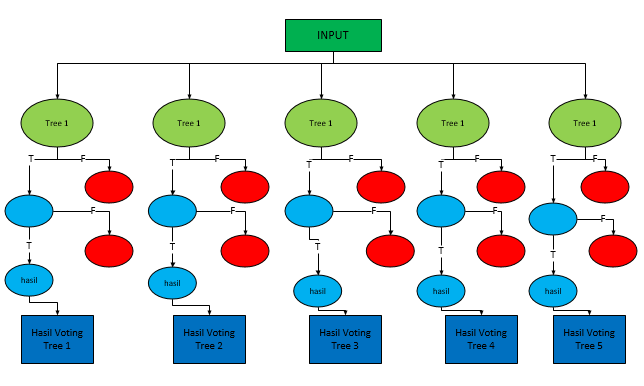
\includegraphics[width=1\textwidth]
      {figures/cokro/c37}}
      \caption{Ilustrasi Voting}
      \label{c37}
      \end{figure}

\begin{figure}
      \centerline{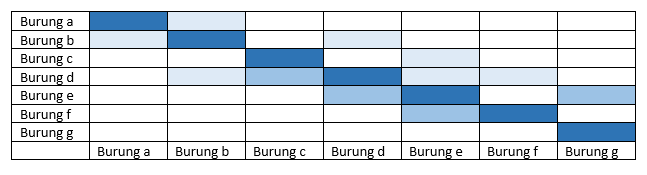
\includegraphics[width=1\textwidth]
      {figures/cokro/c38}}
      \caption{Ilustrasi Confusion matrix}
      \label{c38}
      \end{figure}

\begin{figure}
      \centerline{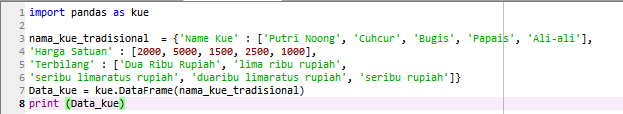
\includegraphics[width=1\textwidth]
      {figures/cokro/c39}}
      \caption{Contoh aplikasi sederhana pandas}
      \label{c39}
      \end{figure}

\begin{figure}
      \centerline{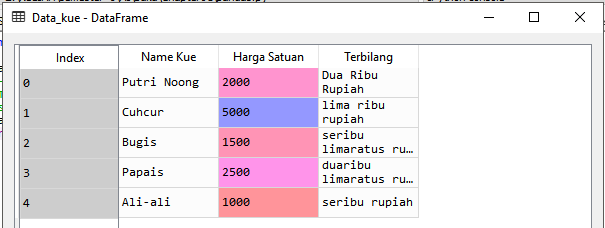
\includegraphics[width=1\textwidth]
      {figures/cokro/c40}}
      \caption{Hasil aplikasi sederhana pandas}
      \label{c40}
      \end{figure}

\begin{figure}
      \centerline{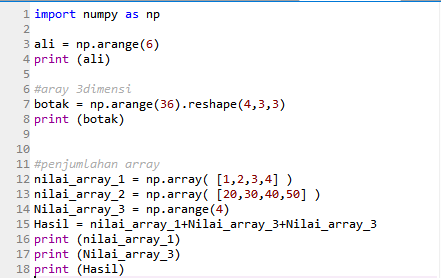
\includegraphics[width=1\textwidth]
      {figures/cokro/c41}}
      \caption{Contoh aplikasi sederhana numpy}
      \label{c41}
      \end{figure}

\begin{figure}
      \centerline{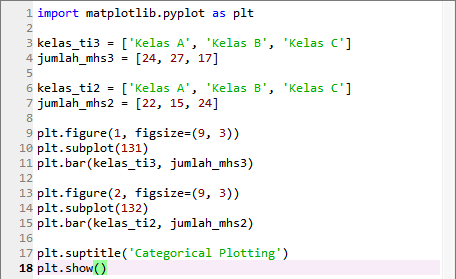
\includegraphics[width=1\textwidth]
      {figures/cokro/c42}}
      \caption{Contoh aplikasi sederhana matplotlib}
      \label{c42}
      \end{figure}

\begin{figure}
      \centerline{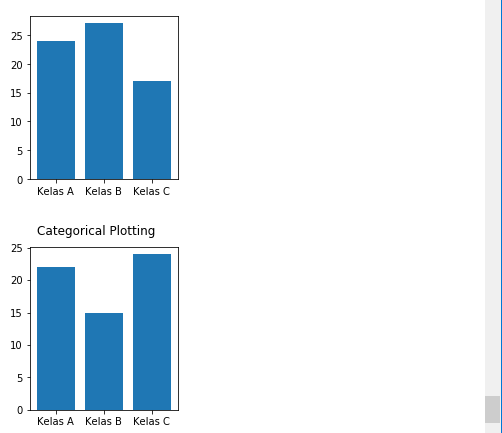
\includegraphics[width=1\textwidth]
      {figures/cokro/c43}}
      \caption{Hasil aplikasi sederhana matplotlib}
      \label{c43}
      \end{figure}

\begin{figure}
      \centerline{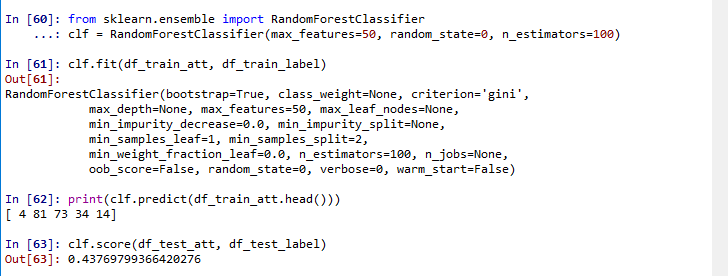
\includegraphics[width=1\textwidth]
      {figures/cokro/c44}}
      \caption{Hasil aplikasi random forest}
      \label{c44}
      \end{figure}

\begin{figure}
      \centerline{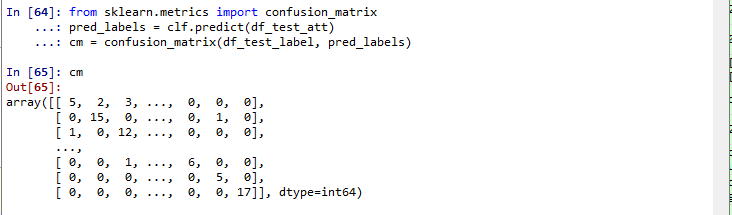
\includegraphics[width=1\textwidth]
      {figures/cokro/c45}}
      \caption{Hasil aplikasi confusion matrix}
      \label{c45}
      \end{figure}

\begin{figure}
      \centerline{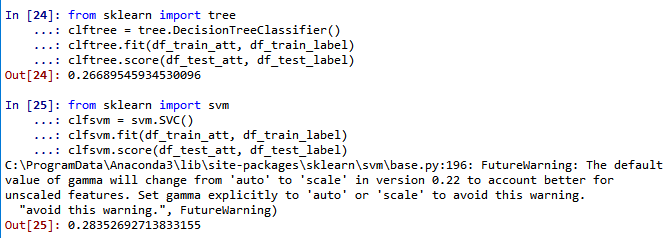
\includegraphics[width=1\textwidth]
      {figures/cokro/c46}}
      \caption{Hasil aplikasi SVM dan Decision tree}
      \label{c46}
      \end{figure}

\begin{figure}
      \centerline{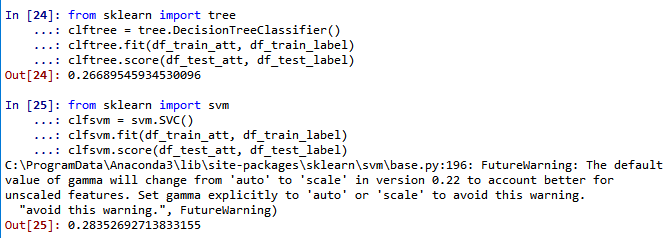
\includegraphics[width=1\textwidth]
      {figures/cokro/c46}}
      \caption{Hasil aplikasi SVM dan Decision tree}
      \label{c46}
      \end{figure}

\begin{figure}
      \centerline{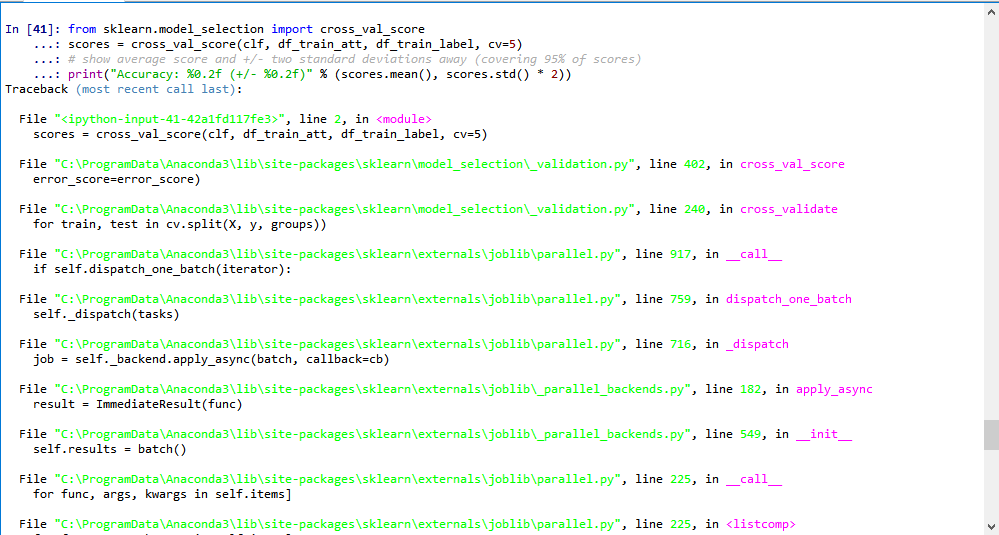
\includegraphics[width=1\textwidth]
      {figures/cokro/c47}}
      \caption{Hasil aplikasi cross validation}
      \label{c47}
      \end{figure}

\begin{figure}
      \centerline{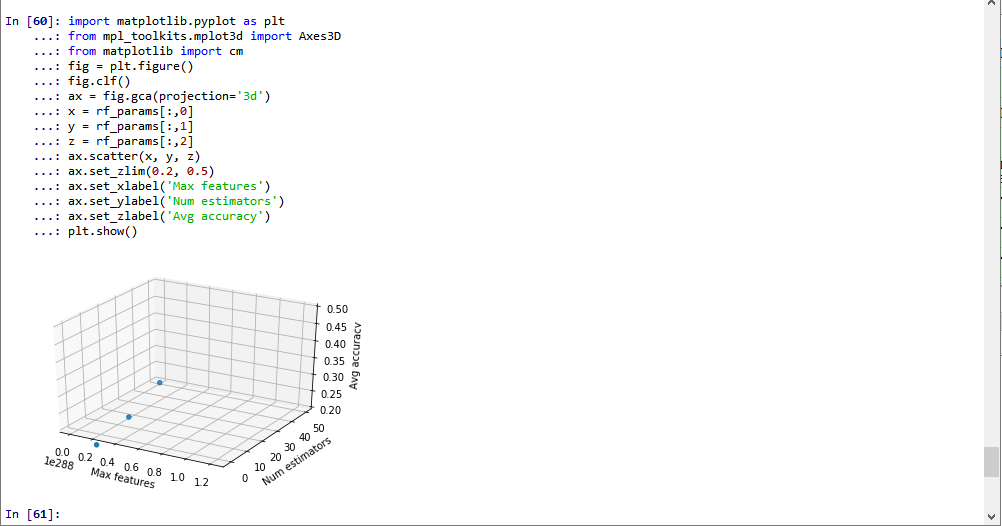
\includegraphics[width=1\textwidth]
      {figures/cokro/c48}}
      \caption{Hasil aplikasi cross validation}
      \label{c48}
      \end{figure}

\begin{figure}
      \centerline{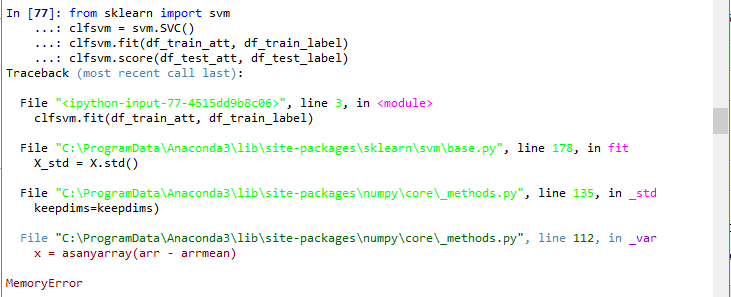
\includegraphics[width=1\textwidth]
      {figures/cokro/c49}}
      \caption{Error Svm}
      \label{c49}
      \end{figure}

\begin{figure}
      \centerline{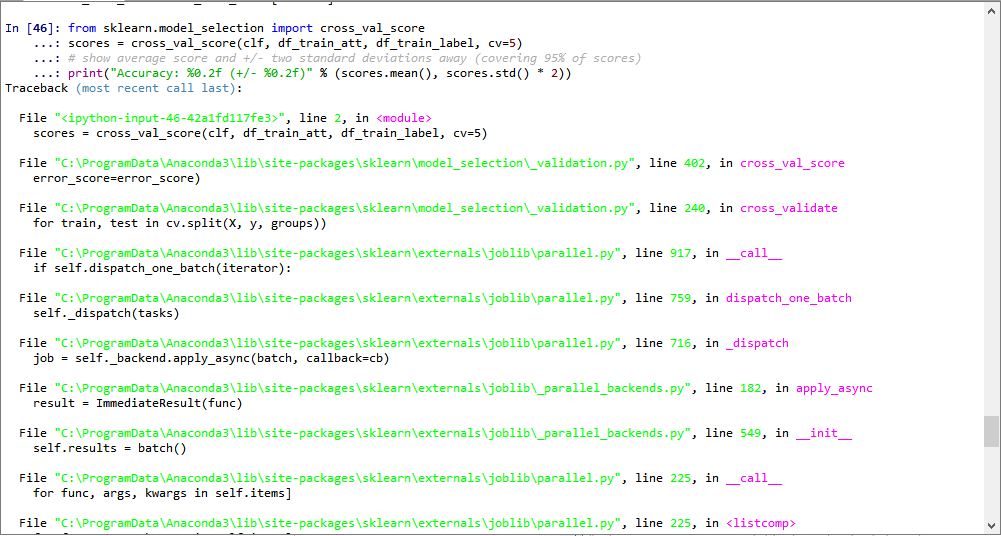
\includegraphics[width=1\textwidth]
      {figures/cokro/c50}}
      \caption{Error Svm}
      \label{c50}
      \end{figure}

\begin{figure}
      \centerline{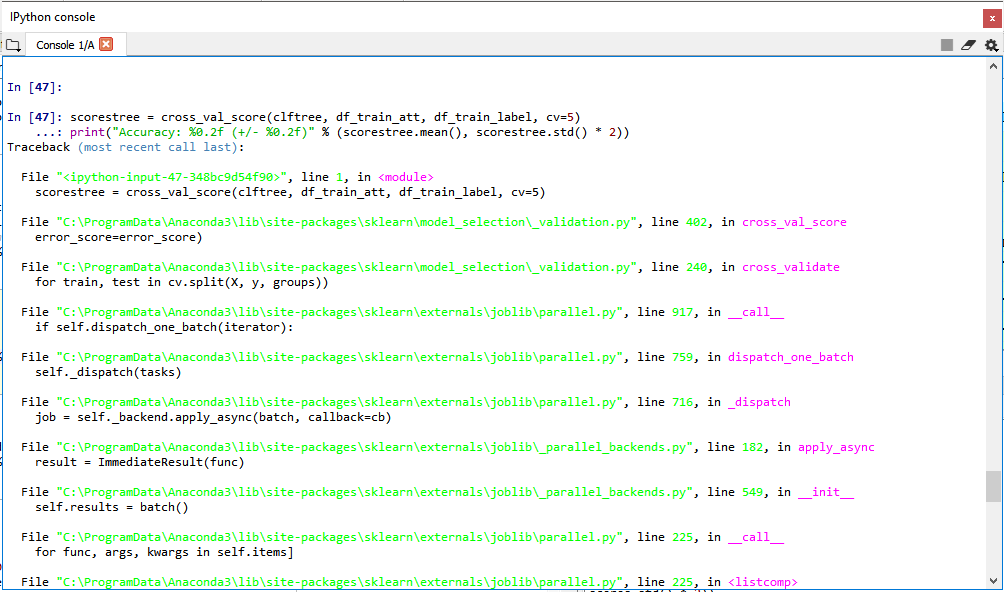
\includegraphics[width=1\textwidth]
      {figures/cokro/c51}}
      \caption{Error Svm}
      \label{c51}
      \end{figure}

\begin{figure}
      \centerline{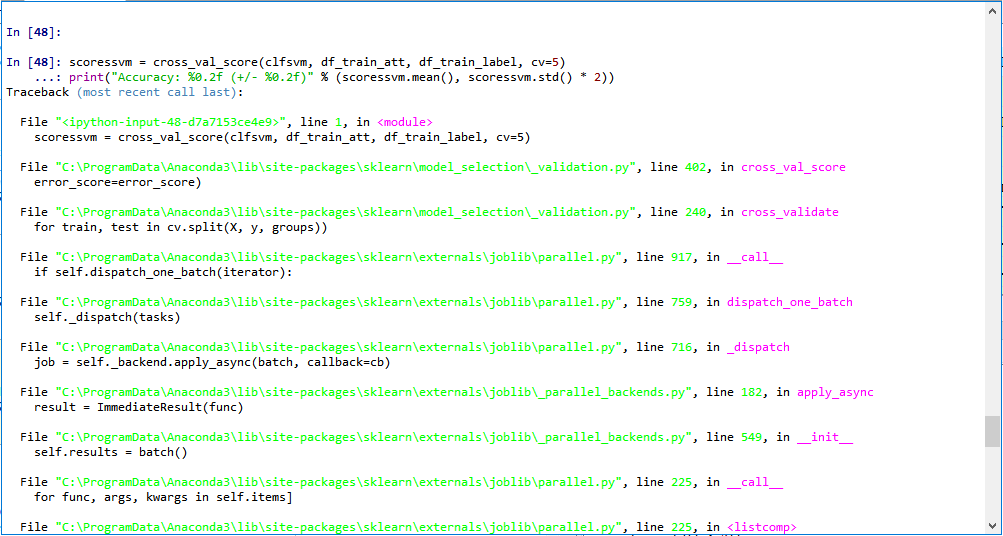
\includegraphics[width=1\textwidth]
      {figures/cokro/c52}}
      \caption{Error Svm}
      \label{c52}
      \end{figure}

\begin{figure}
      \centerline{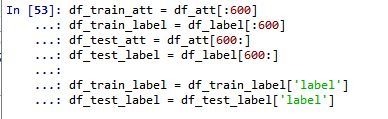
\includegraphics[width=1\textwidth]
      {figures/cokro/c53}}
      \caption{Merubah data training}
      \label{c53}
      \end{figure}

\begin{figure}
      \centerline{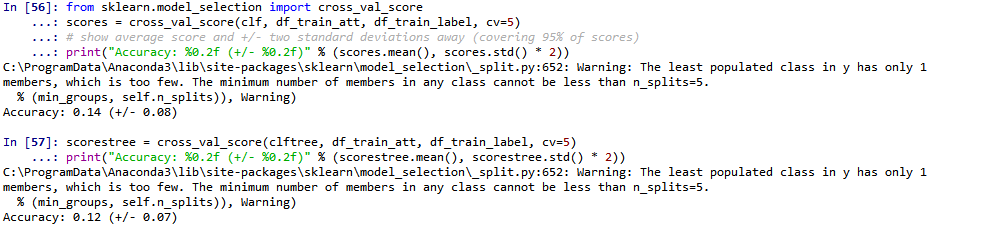
\includegraphics[width=1\textwidth]
      {figures/cokro/c54}}
      \caption{Hasil Solusi}
      \label{c54}
      \end{figure}


\section{Ahmad Syafrizal Huda / 1164062}
\subsection{Teori}
\begin{enumerate}
\item Random forest ialah sekumpulan classifier yang terdiri dari banyak pohon keputusan dan mengerjakan klasifikasi berdasarkan keluaran dari hasil klasifikasi setiap pohon keputusan anggota. Klasifikasi random forest dikerjakan melalui penggabungan pohon (tree) dengan melakukan training pada sampel data yang dimiliki. Contoh ilustrasi gambar random forest pada gambar \ref{h1}.
\item Cara membaca dataset kasus dan makna setiap file dan isi field masing-masing file
\subitem Gunakan librari pandas yang sudah di install sebelumnya pada python untuk dapat membaca dataset dengan format text file.
\subitem  Selanjutnya buatlah variabel baru misalkan diberi nama dataset yang berisikan perintah untuk membaca file csv.
\begin{verbatim}
import pandas as data
dataset = data.read_csv("car.txt")
dataset.head()
\end{verbatim}
\subitem Pada perintah diatas yaitu memanggil library pandas untuk membaca dataset, membuat variabel dataset yang berisikan data.read\_csv untuk membaca dataset. Pada contoh ini menggunakan txt tapi tetap bisa membaca datasetnya, karena pada saat dijalankan librari pandas secara otomatis akan mengubah data dalam bentuk text file ke format csv. Hasilnya seperti pada gambar \ref{h2}.
\subitem Penjelasan dari isi field pada hasil gambar \ref{h2} yaitu: Atribut Index merupakan atribut otomatis untuk penomoran data yang sudah ada, Atribut Buying merupakan harga beli dari mobil tersebut. dengan value : v high/Sangat mahal,high/mahal,med/Cukup, low/Murah, Atribut Maint merupakan harga perawatan dari mobil tersebut, dengan value sama seperti pada atribut Buying, Atribut Doors merupakan jumlah pintu yang terdapat pada mobil, dengan value 2,3,4,5 more atau lebih dari 5, Atribut Persons merupakan kapasitas orang yang bisa masuk kedapalm mobil, dengan value 2,4, more /lebih, Atribut Lug Boot merupakan ukuran bagasi boot mobil, dengan value small,med,big, Atribut Safety merupakan perkiraan keselamatan mobil, dengan value low,med,high, Yang terakhir yaitu Value, yang dimana merupakan merupakan Class nya atau disebut dengan targetnya menyatakan apakah mobil tersebut dapat diterima atau tidak dan apakah mobil tersebut bagus atau tidak, dengan value unacc, acc, good,v good.
\item Cross validation adalah teknik validasi model untuk menilai bagaimana hasil analisis statistik (model) akan digeneralisasi ke kumpulan data independen. Ini terutama digunakan dalam pengaturan di mana tujuannya adalah prediksi, dan orang ingin memperkirakan seberapa akurat model prediksi akan dilakukan dalam praktek.
\item Arti score 44\% pada random forest yaitu merupakan outputannya untuk hutan acak, arti score 27\% pada decission tree adalah presentasi hasil dari perhitungan dataset acak, dan arti score 29\% dari SVM adalah hasil pendekatan jaringan saraf.  Hasil tersebut didapat dari hasil valdasi silang untuk memastikan bahwa membagi training test dengan cara yang berbeda. Jadi 44\% untuk random forest, 27\% untuk pohon keputusan, dan 29\% untuk SVM. Itu merupakan presentase keakurasian prediksi yang dilakukan pada saat testing menggunakan label pada dataset yang digunakan. Score mendefinisikan aturan evaluasi model.
\item Perhitungan confusion Matriks dapat dilakukan sebagai berikut:
\subitem Import librari Pandas, Matplotlib, dan Numpy.
\subitem Buat variabel x\_aktu yang berisikan data aktual.
\subitem Buat variabel x\_diksi berisikan data yang akan dijadikan sebagai prediksi.
\subitem Buat variabel ak\_confusion yang berisikan crosstab untuk membangun tabel tabulasi silang yang dapat menunjukkan frekuensi kemunculan kelompok data tertentu.
\subitem Pada variabel ak\_confusion definisikan lagi nama baris yaitu Aktual dan kolomnya Prediksi
\subitem Kemudian definisikan suatu fungsi yang diberi nama plot confusion matrix yang berisikan pendefinisian confusion matrix dan juga akan di plotting. untuk code perintah lengkapnya sebagai berikut :
\subitem
\begin{verbatim}
import numpy as cm1
import matplotlib.pyplot as plt
import pandas as cm2
x_aktu = cm2.Series([3, 1, 3, 3, 1, 2, 2, 3, 3, 1, 2, 3], name='Aktual')
x_diksi = cm2.Series([1, 1, 3, 2, 1, 3, 2, 1, 3, 1, 3, 3], name='Prediksi')
ak_confusion = cm2.crosstab(x_aktu, x_diksi)
ak_confusion = cm2.crosstab(x_aktu, x_diksi, rownames=['Aktual'], colnames=['Prediksi'], margins=True)
def plot_confusion_matrix(df_confusion, title='Confusion matrix', cmap=plt.cm.gray_r):
    plt.matshow(ak_confusion, cmap=cmap) # imshow
    #plt.title(title)
    plt.colorbar()
    tick_marks = cm1.arange(len(ak_confusion.columns))
    plt.xticks(tick_marks, ak_confusion.columns, rotation=45)
    plt.yticks(tick_marks, ak_confusion.index)
    #plt.tight_layout()
    plt.ylabel(ak_confusion.index.name)
    plt.xlabel(ak_confusion.columns.name)
plot_confusion_matrix(ak_confusion)
plt.show()
\end{verbatim}
Hasilnya akan seperti pada gambar \ref{h3} :
\item Voting pada random forest sebagaimana voting yaitu suara/hasil untuk setiap target yang diprediksi pada saat melakukan Random Forest. Pertimbangkan target prediksi dengan voting terbanyak/tertinggi sebagai prediksi akhir dari algoritma random forest. Contoh ilustrasi dapat dilihat pada gambar \ref{h4}.
\end{enumerate}

\subsection{Praktek Program}
\begin{enumerate}
\item 
\begin{verbatim}
import pandas as huda
a = huda.Series(['Ahmad', 'Syaf', 'Rizal', 'Huda', 'Mubarrok'],
index = [1, 2, 3, 4, 5])
print (a)
\end{verbatim}
\subitem Baris pertama pada codingan, yaitu import pandas as huda yang artinya kita akan mengimport librari pandas dari python dengan inisiasi huda.
\subitem Baris kedua pada codingan, yaitu Variabel a didefinisikan data data yang sudah dibuat seperti daftar nama dengan menggunakan huda.Series. Series adalah object satu dimensi yang serupa dengan kolom di dalam tabel.
\subitem Baris ketiga pada codingan, yaitu index digunakan untuk melabeli data dengan dimulai dari nomor 1...5, jika tidak label default akan dimulai dari 0,1,2...
\subitem Baris keempat pada codingan, yaitu digunakan untuk mencetak atau menampilkan data pada variabel a yang sudah dibuat sebelumnya.
\subitem Untuk hasilnya dapat dilihat pada gambar \ref{h5}.
\item 
\begin{verbatim}
import numpy as huda
print (huda.arange(50, 101)) 
\end{verbatim}
\subitem Baris pertama pada codingan, yaitu import numpy as huda yang artinya kita akan mengimport librari numpy dari python dengan inisiasi huda.
\subitem Baris kedua pada codingan, yaitu digunakan untuk mencetak atau menampilkan data dengan menggunakan huda.arange untuk membuat array dengan bilangan sekuensial dari mulai nilai awal 50 sampai sebelum 101 dengan berurutan.
\subitem Untuk hasilnya dapat dilihat pada gambar \ref{h6}.
\item 
\begin{verbatim}
import matplotlib.pyplot as huda
huda.plot([0,1,3,5,7,8,10],[25, 35, 30, 45, 50, 45, 30])
huda.show()
\end{verbatim}
\subitem Baris pertama pada codingan, yaitu import matplotlib.pyplot as huda yang artinya kita akan mengimport librari matplotlib dengan class pyplot dari python dengan inisiasi huda.
\subitem Baris kedua pada codingan, yaitu digunakan untuk memasukkan data dengan insiai huda pada class plot dengan nilai x dan y yg sudah ditentukkan.
\subitem Baris ketiga pada codingan, yaitu digunakan untuk mencetak atau menampilkan data dengan inisiai huda.show nantinya keluaranyya berupa grafik.
\subitem Untuk hasilnya dapat dilihat pada gambar \ref{h7}.

\item Menjalankan Klasifikasi Random Forest.
\subitem Pada gambar \ref{h8} berfungsi untuk membaca data yang berupa image\_attribute\_labels dengan format text file. Dengan mendefinisikan variabel imgatt yang berisikan value untuk membaca data, juga menggunakan code untuk skip data yang mengandung bad lines agar tidak terjadi eror pada saat pembacaan file.
\subitem Pada gambar \ref{h9} yaitu mengembalikan baris n teratas (5 secara default) dari dataframe imgatt.
\subitem Pada gambar \ref{h10} yaitu menampilkan beberapa baris dan kolom dari dataframe imgatt.
\subitem Pada gambar \ref{h11} yaitu variabel imgatt2 menggunakan function pivot untuk mengubah kolom jadi baris, dan baris jadi kolom dari dataframe sebelumnya.
\subitem Pada gambar \ref{h12} yaitu imgatt2 head berfungsi untuk mengembalikan nilai teratas dari dataframe imgatt2.
\subitem Pada gambar \ref{h13} yaitu menampilkan beberapa baris dan kolom dari dataframe imgatt2. 
\subitem Pada gambar \ref{h14} yaitu melakukan pivot yang mana imgid menjadi index yang artinya unik.
\subitem Pada gambar \ref{h15} yaitu memuat jawabannya yang berisi apakah burung itu termasuk dalam spesies yang mana. Dua kolomnya terdiri dari imgid dan label.
\subitem Pada gambar \ref{h16} yaitu menunjukkan 11788 baris dan 1 kolom. Dimana kolom itu adalah jenis spesies burungnya.
\subitem Pada gambar \ref{h17} yaitu join antara imgatt2 dengan imglabels dikarenakan isinya sama. Sehingga kita bisa mendapatkan data ciri dan data jawabannya/labelnya sehingga bisa dikategorikan supervised learning.
\subitem Pada gambar \ref{h18} yaitu menghilangkan label yang didepan, dan menggunakan label yang paling belakang yang baru di join.
\subitem Pada gambar \ref{h19} yaitu mengecek 5 data teratas dari df att.
\subitem Pada gambar \ref{h20} yaitu mengecek 5 data teratas dari df label.
\subitem Pada gambar \ref{h21} yaitu 8000 row pertama sebagai data training sisanya sebagai data testing dengan membagi menjadi dua bagian.
\subitem Pada gambar \ref{h22} yaitu memanggil kelas RandomForestClassifier. max features diartikan sebagai berapa banyak kolom pada setiap tree dengan isi maksimum 50.
\subitem Pada gambar \ref{h23} yaitu melakukan fit untuk membangun random forest yang sudah ditentukan dengan maksimum fitur sebanya 50 untuk perpohonnya.
\subitem Pada gambar \ref{h24} yaitu menampilkan hasil prediksi dari random forest sebelumnya.
\subitem Pada gambar \ref{h25} yaitu menampilkan besaran akurasinya dari prediksi diatas atau score perolehan dari klasifikasi.

\item Menjalankan Confusion Matrix.
\subitem Pada gambar \ref{h26} yaitu menyatukan Random Forest ke dalam Confusion Matrix
\subitem Pada gambar \ref{h27} yaitu menampilkan hasil dari gambar sebekumnya dengan array pada perintah cm.
\subitem Pada gambar \ref{h28} yaitu Plotting Confusion Matrix dengan librari Matplotlib.
\subitem Pada gambar \ref{h29} yaitu Set plot sumbunya sesuai dengan nama datanya dan membaca file classes.txt.
\subitem Pada gambar \ref{h30} yaitu Plot hasil perubahan label yang sudah dilakukan.

\item Menjalankan Klasifikasi SVM dan Decision Tree.
\subitem Pada gambar \ref{h31} yaitu klasifikasi dengan decission tree dengan dataset yang sama dan akan muncul akurasi prediksinya.
\subitem Pada gambar \ref{h32} yaitu  klasifikasi dengan SVM dengan dataset yang sama dan akan muncul akurasi prediksinya.
\item Menjalankan Cross Validation.
\subitem Pada gambar \ref{h33} yaitu Cross Validation untuk  Random Forest.
\subitem Pada gambar \ref{h34} yaitu Cross Validation untuk Decission Tree.
\subitem Pada gambar \ref{h35} yaitu Cross Validation untuk SVM.
\item Menjalankan Pengamatan Komponen Informasi.
\subitem Pada gambar \ref{h36} yaitu untuk mengetahui berapa banyak tree yang dibuat, berapa banyak atribut yang dipakai dan informasi lainnya.
\subitem Pada gambar \ref{h37} yaitu hasil dari plotting komponen informasi agar dapat dibaca.
\end{enumerate}

\subsection{Penanganan Eror}
\begin{enumerate}
\item Screenshootan eror ada pada gambar \ref{h38}.
\item 
\begin{verbatim}
from sklearn.model_selection import cross_val_score
scores = cross_val_score(clf, df_train_att, df_train_label, cv=5)
print("Accuracy: %0.2f (+/- %0.2f)" % (scores.mean(), scores.std() * 2))
\end{verbatim}
\subitem 
\begin{verbatim}
scorestree = cross_val_score(clftree, df_train_att, df_train_label, cv=5)
print("Accuracy: %0.2f (+/- %0.2f)" % (scorestree.mean(), scorestree.std() * 2))
\end{verbatim}
\subitem 
\begin{verbatim}
scoressvm = cross_val_score(clfsvm, df_train_att, df_train_label, cv=5)
print("Accuracy: %0.2f (+/- %0.2f)" % (scoressvm.mean(), scoressvm.std() * 2))
\end{verbatim}
\subitem 
\begin{verbatim}
max_features_opts = range(1, 10, 1)
n_estimators_opts = range(2, 40, 4)
rf_params = np.empty((len(max_features_opts)*len(n_estimators_opts),4), float)
i = 0
for max_features in max_features_opts:
    for n_estimators in n_estimators_opts:
        clf = RandomForestClassifier(max_features=max_features, n_estimators=n_estimators)
        scores = cross_val_score(clf, df_train_att, df_train_label, cv=5)
        rf_params[i,0] = max_features
        rf_params[i,1] = n_estimators
        rf_params[i,2] = scores.mean()
        rf_params[i,3] = scores.std() * 2
        i += 1
        print("Max features: %d, num estimators: %d, accuracy: %0.2f (+/- %0.2f)" %
\end{verbatim}
\item Solusi pemecahan masalah tersebut yaitu dengan cara mengubah pada codingan dibawah in yang awalnya datanya 8000 menjadi 1000 semua dan max\_featurenya awalnya 50 menjadi 25.
\subitem 
\begin{verbatim}
df_train_att = df_att[:1000]
df_train_label = df_label[:1000]
df_test_att = df_att[1000:]
df_test_label = df_label[1000:]

df_train_label = df_train_label['label']
df_test_label = df_test_label['label']

from sklearn.ensemble import RandomForestClassifier
clf = RandomForestClassifier(max_features=25, random_state=0, n_estimators=100)
\end{verbatim}
\subitem Jika sudah dilakukan maka langkah selanjutnya yaitu kita tinggal merunning ulang dari awal hingga data tersebut berhasil diajalankan
\end{enumerate}

\begin{figure}
	\centerline{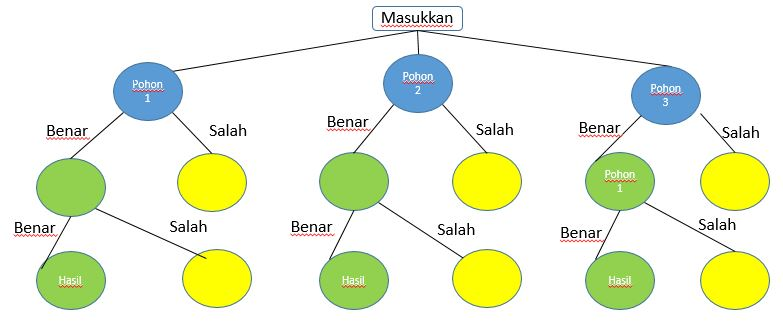
\includegraphics[width=1\textwidth]{figures/huda/chapter3/1.JPG}}
	\caption{Random Forest}
	\label{h1}
\end{figure}

\begin{figure}
	\centerline{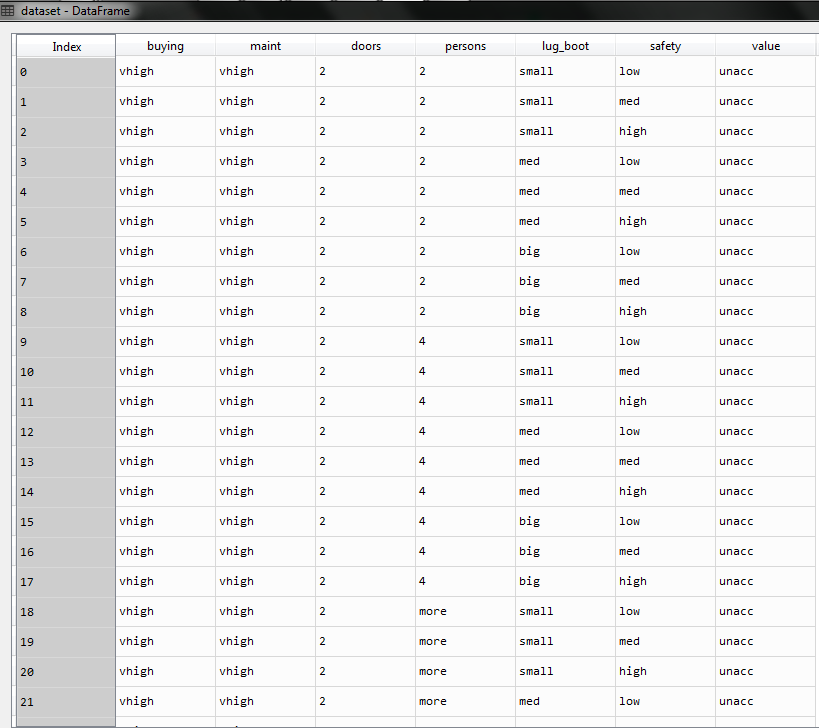
\includegraphics[width=1\textwidth]{figures/huda/chapter3/2.PNG}}
	\caption{Hasil Dataset}
	\label{h2}
\end{figure}

\begin{figure}
	\centerline{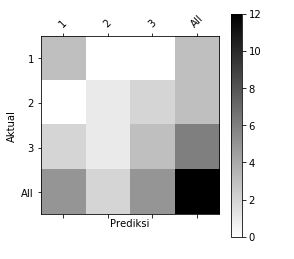
\includegraphics[width=1\textwidth]{figures/huda/chapter3/3.JPG}}
	\caption{Confusion Matrix}
	\label{h3}
\end{figure}

\begin{figure}
	\centerline{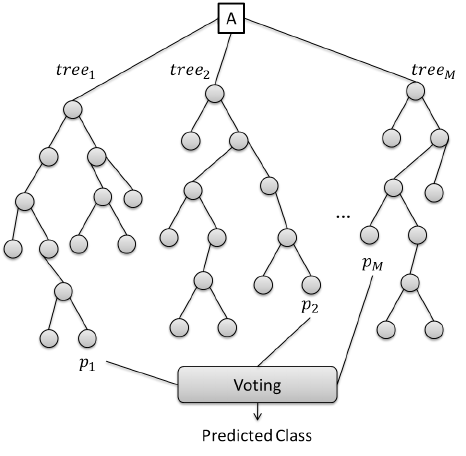
\includegraphics[width=1\textwidth]{figures/huda/chapter3/4.png}}
	\caption{Voting}
	\label{h4}
\end{figure}

\begin{figure}
	\centerline{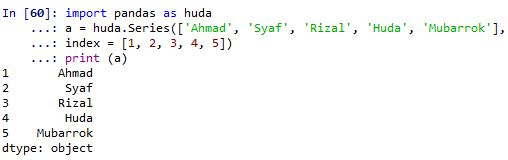
\includegraphics[width=1\textwidth]{figures/huda/chapter3_praktek/1.JPG}}
	\caption{Aplikasi Menggunakan Pandas}
	\label{h5}
\end{figure}

\begin{figure}[ht]
	\centerline{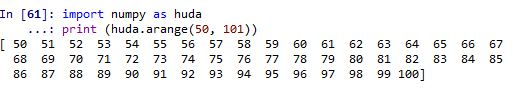
\includegraphics[width=1\textwidth]{figures/huda/chapter3_praktek/2.JPG}}
	\caption{Aplikasi Menggunakan Numpy}
	\label{h6}
\end{figure}

\begin{figure}[ht]
	\centerline{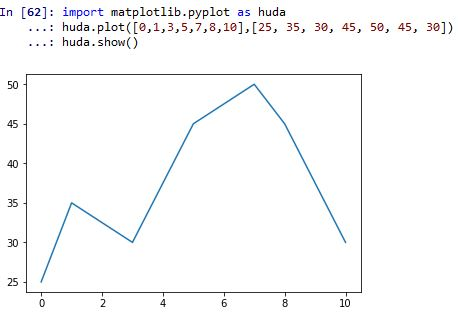
\includegraphics[width=1\textwidth]{figures/huda/chapter3_praktek/3.JPG}}
	\caption{Aplikasi Menggunakan Matplotlib}
	\label{h7}
\end{figure}

\begin{figure}[ht]
	\centerline{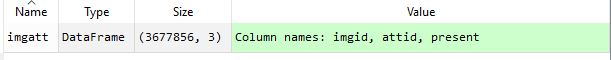
\includegraphics[width=1\textwidth]{figures/huda/chapter3_praktek/4.JPG}}
	\caption{Hasil 1 Random Forest}
	\label{h8}
\end{figure}

\begin{figure}[ht]
	\centerline{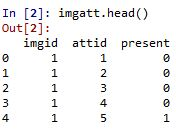
\includegraphics[width=1\textwidth]{figures/huda/chapter3_praktek/5.JPG}}
	\caption{Hasil 2 Random Forest}
	\label{h9}
\end{figure}

\begin{figure}[ht]
	\centerline{\includegraphics[width=1\textwidth]{figures/huda/chapter3_praktek/6.JPG}}
	\caption{Hasil 3 Random Forest}
	\label{h10}
\end{figure}

\begin{figure}[ht]
	\centerline{\includegraphics[width=1\textwidth]{figures/huda/chapter3_praktek/7.JPG}}
	\caption{Hasil 4 Random Forest}
	\label{h11}
\end{figure}

\begin{figure}[ht]
	\centerline{\includegraphics[width=1\textwidth]{figures/huda/chapter3_praktek/8.JPG}}
	\caption{Hasil 5 Random Forest}
	\label{h12}
\end{figure}

\begin{figure}[ht]
	\centerline{\includegraphics[width=1\textwidth]{figures/huda/chapter3_praktek/9.JPG}}
	\caption{Hasil 6 Random Forest}
	\label{h13}
\end{figure}

\begin{figure}[ht]
	\centerline{\includegraphics[width=1\textwidth]{figures/huda/chapter3_praktek/10.JPG}}
	\caption{Hasil 7 Random Forest}
	\label{h14}
\end{figure}

\begin{figure}[ht]
	\centerline{\includegraphics[width=1\textwidth]{figures/huda/chapter3_praktek/11.JPG}}
	\caption{Hasil 8 Random Forest}
	\label{h15}
\end{figure}

\begin{figure}[ht]
	\centerline{\includegraphics[width=1\textwidth]{figures/huda/chapter3_praktek/12.JPG}}
	\caption{Hasil 9 Random Forest}
	\label{h16}
\end{figure}

\begin{figure}[ht]
	\centerline{\includegraphics[width=1\textwidth]{figures/huda/chapter3_praktek/13.JPG}}
	\caption{Hasil 10 Random Forest}
	\label{h17}
\end{figure}

\begin{figure}[ht]
	\centerline{\includegraphics[width=1\textwidth]{figures/huda/chapter3_praktek/14.JPG}}
	\caption{Hasil 11 Random Forest}
	\label{h18}
\end{figure}

\begin{figure}[ht]
	\centerline{\includegraphics[width=1\textwidth]{figures/huda/chapter3_praktek/15.JPG}}
	\caption{Hasil 11 Random Forest}
	\label{h19}
\end{figure}

\begin{figure}[ht]
	\centerline{\includegraphics[width=1\textwidth]{figures/huda/chapter3_praktek/16.JPG}}
	\caption{Hasil 12 Random Forest}
	\label{h20}
\end{figure}

\begin{figure}[ht]
	\centerline{\includegraphics[width=1\textwidth]{figures/huda/chapter3_praktek/17.JPG}}
	\caption{Hasil 13 Random Forest}
	\label{h21}
\end{figure}

\begin{figure}[ht]
	\centerline{\includegraphics[width=1\textwidth]{figures/huda/chapter3_praktek/18.JPG}}
	\caption{Hasil 14 Random Forest}
	\label{h22}
\end{figure}

\begin{figure}[ht]
	\centerline{\includegraphics[width=1\textwidth]{figures/huda/chapter3_praktek/19.JPG}}
	\caption{Hasil 15 Random Forest}
	\label{h23}
\end{figure}

\begin{figure}[ht]
	\centerline{\includegraphics[width=1\textwidth]{figures/huda/chapter3_praktek/20.JPG}}
	\caption{Hasil 16 Random Forest}
	\label{h24}
\end{figure}

\begin{figure}[ht]
	\centerline{\includegraphics[width=1\textwidth]{figures/huda/chapter3_praktek/21.JPG}}
	\caption{Hasil 17 Random Forest}
	\label{h25}
\end{figure}

\begin{figure}[ht]
	\centerline{\includegraphics[width=1\textwidth]{figures/huda/chapter3_praktek/22.JPG}}
	\caption{Hasil 1 Confusion Matrix}
	\label{h26}
\end{figure}

\begin{figure}[ht]
	\centerline{\includegraphics[width=1\textwidth]{figures/huda/chapter3_praktek/23.JPG}}
	\caption{Hasil 2 Confusion Matrix}
	\label{h27}
\end{figure}

\begin{figure}[ht]
	\centerline{\includegraphics[width=1\textwidth]{figures/huda/chapter3_praktek/24.JPG}}
	\caption{Hasil 3 Confusion Matrix}
	\label{h28}
\end{figure}

\begin{figure}[ht]
	\centerline{\includegraphics[width=1\textwidth]{figures/huda/chapter3_praktek/25.JPG}}
	\caption{Hasil 4 Confusion Matrix}
	\label{h29}
\end{figure}

\begin{figure}[ht]
	\centerline{\includegraphics[width=1\textwidth]{figures/huda/chapter3_praktek/26.JPG}}
	\caption{Hasil 5 Confusion Matrix}
	\label{h30}
\end{figure}

\begin{figure}[ht]
	\centerline{\includegraphics[width=1\textwidth]{figures/huda/chapter3_praktek/27.JPG}}
	\caption{Hasil 1 Klasifikasi SVM dan Decision Tree}
	\label{h31}
\end{figure}

\begin{figure}[ht]
	\centerline{\includegraphics[width=1\textwidth]{figures/huda/chapter3_praktek/28.JPG}}
	\caption{Hasil 2 Klasifikasi SVM dan Decision Tree}
	\label{h32}
\end{figure}

\begin{figure}[ht]
	\centerline{\includegraphics[width=1\textwidth]{figures/huda/chapter3_praktek/29.JPG}}
	\caption{Hasil 1 Cross Validation}
	\label{h33}
\end{figure}

\begin{figure}[ht]
	\centerline{\includegraphics[width=1\textwidth]{figures/huda/chapter3_praktek/30.JPG}}
	\caption{Hasil 2 Cross Validation}
	\label{h34}
\end{figure}

\begin{figure}[ht]
	\centerline{\includegraphics[width=1\textwidth]{figures/huda/chapter3_praktek/31.JPG}}
	\caption{Hasil 3 Cross Validation}
	\label{h35}
\end{figure}

\begin{figure}[ht]
	\centerline{\includegraphics[width=1\textwidth]{figures/huda/chapter3_praktek/32.JPG}}
	\caption{Hasil 1 Pengamatan Komponen Informasi}
	\label{h36}
\end{figure}

\begin{figure}[ht]
	\centerline{\includegraphics[width=1\textwidth]{figures/huda/chapter3_praktek/33.JPG}}
	\caption{Hasil 2 Pengamatan Komponen Informasi}
	\label{h37}
\end{figure}

\begin{figure}[ht]
	\centerline{\includegraphics[width=1\textwidth]{figures/huda/chapter3_praktek/eror.JPG}}
	\caption{Eror}
	\label{h38}
\end{figure}